\section{Fluctuations}
\begin{frame} {Fluctuations}
    \begin{itemize}
        \item Turbulent fluctuations produce an $\mathbf{E\times B}$ drift velocity $\delta v_\perp = \delta E_\perp/B$.
        \item With density fluctuation $\delta n$, the convective particle flux is
              \[ \Gamma = \expval{\delta v_\perp\delta n} \]
              Average is taken over the flux surface.
        \item With magnetic fluctuations $\delta \mathbf{B}$, the flux is
              \[ \Gamma_j = \frac{n}{B}\expval{\delta v_{\parallel j}\delta B_r} \]
    \end{itemize}
\end{frame}

\begin{frame} {Fluctuations and $\tau_E$}
    \begin{figure}
        \centering
        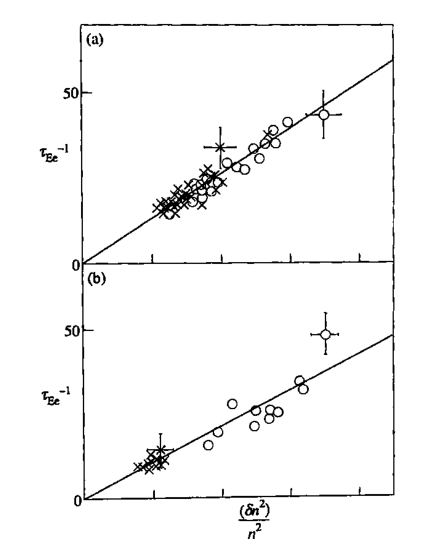
\includegraphics[width=0.35\textwidth]{figures/fluctuations-and-tau-e.png}
        \caption{Measurements from TFR showing a correlation between the level of density fluctuations and the electron energy confinement time (with allowance for the effect of sawtooth oscillations). Figure (a) is for ion cyclotron heating and Fig.(b) is for neutral beam beating. Both figures also give results for ohmic heating.}
        \label{fig:}
    \end{figure}
\end{frame}

\begin{frame} {Fluctuations and L-H Transition}
    \begin{figure}
        \centering
        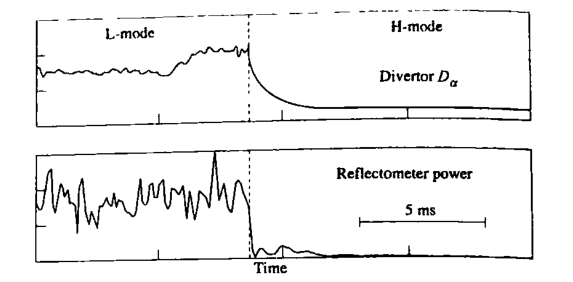
\includegraphics[width=0.7\textwidth]{figures/fluctuations-and-modes.png}
        \caption{Showing the fall of density fluctuations as measured by reflectometry during an L-H transition in DIII-D.}
        \label{fig:fluctuation-and-modes}
    \end{figure}
\end{frame}

\begin{frame} {Turbulence-Induced Transport}
    \begin{itemize}
        \item \textbf{Transport due to electrostatic fluctuations}:
              \[ D = \sum_k \left( \frac{k_\perp\delta\phi_k}{B} \right)^2 \tau_k \]
              We have assumed the fluctuations of electric potential $\delta\phi = \sum_k\delta\phi_ke^{i\mathbf{k\cdot x}}$. The time variation of the fluctuation is characterized by $\tau_k \sim 1/\omega_k$.
        \item \textbf{Transport due to magnetic fluctuations}:
              \[ D_M = \sum_k \frac{k_\perp\omega_k^3}{L_s} \]
    \end{itemize}
\end{frame}